\documentclass[paper=a4, fontsize=11pt]{scrartcl} % A4 paper and 11pt font size

\usepackage[T1]{fontenc} % Use 8-bit encoding that has 256 glyphs
\usepackage[english]{babel} % English language/hyphenation
\usepackage{amsmath,amsfonts,amsthm} % Math packages
\usepackage{graphicx}
\usepackage{sectsty} % Allows customizing section commands
\usepackage{listings}
\usepackage{hyperref}
\usepackage{float}
\usepackage{placeins}
\usepackage{subcaption}
\usepackage{cleveref}
\usepackage{multimedia}

\allsectionsfont{ \normalfont\scshape} % Make all sections centered, the default font and small caps

\usepackage{fancyhdr} % Custom headers and footers
\pagestyle{fancyplain} % Makes all pages in the document conform to the custom headers and footers
\fancyhead{} % No page header - if you want one, create it in the same way as the footers below
\fancyfoot[L]{} % Empty left footer
\fancyfoot[C]{} % Empty center footer
\fancyfoot[R]{\thepage} % Page numbering for right footer
\renewcommand{\headrulewidth}{0pt} % Remove header underlines
\renewcommand{\footrulewidth}{0pt} % Remove footer underlines
\setlength{\headheight}{13.6pt} % Customize the height of the header


%----------------------------------------------------------------------------------------
%	TITLE SECTION
%----------------------------------------------------------------------------------------

\newcommand{\horrule}[1]{\rule{\linewidth}{#1}} % Create horizontal rule command with 1 argument of height

\title{	
\normalfont \normalsize 
\textsc{Indian Institute of Technology Delhi} \\ [25pt] % Your university, school and/or department name(s)
\horrule{0.5pt} \\[0.4cm] % Thin top horizontal rule
\huge Image Rectification \\ % The assignment title
\horrule{2pt} \\[0.5cm] % Thick bottom horizontal rule
}

\author{Suyash Agrawal \\ 2015CS10262} % Your name

\date{\normalsize\today} % Today's date or a custom date

\begin{document}

\maketitle % Print the title

\section{Introduction}
In this assignment we implemented image rectification, namely, affine rectification and metric rectification.
The user select four points in image which should lie in a rectange and it outpus the rectified images.

\section{Affine Rectification}
Affine rectification was done using the following algorithm:
\begin{itemize}
    \item Using the selected points we construct two pairs of lines which should have been parallel in eucledian space.
    \item Next we calculated the intersection points of these lines in the image space.
    \item Using these intersection points we calculated the line at infinity in the image.
    \item Then we constructed a homography which transforms line at infinity to its canonical form.
    \item This is the homography that we then use to affine rectify the image. 
\end{itemize}

\section{Metric Rectification}
For Metric rectification we used the following method:
\begin{itemize}
    \item We constructed a rectangle located approximately at the image conordinates of the selected points.
    \item We then constructed a projective transformation that transformed the input points by the user to the
          points of the constructed rectangle
    \item This is the homography that we then use to metric rectify the image.
\end{itemize}

This method is sound because the transformation that maps the input points to the rectangle, actually
moves the conic dual to circular points to its canonical location in the metric corrected image.

\section{Results}
We ran the program on a sample set of images which were freely available in the internet (Google image search).
Some of the the results are given below:
  \begin{figure*}
    \centering
    \begin{subfigure}[ht]{0.3\textwidth}
        \centering
        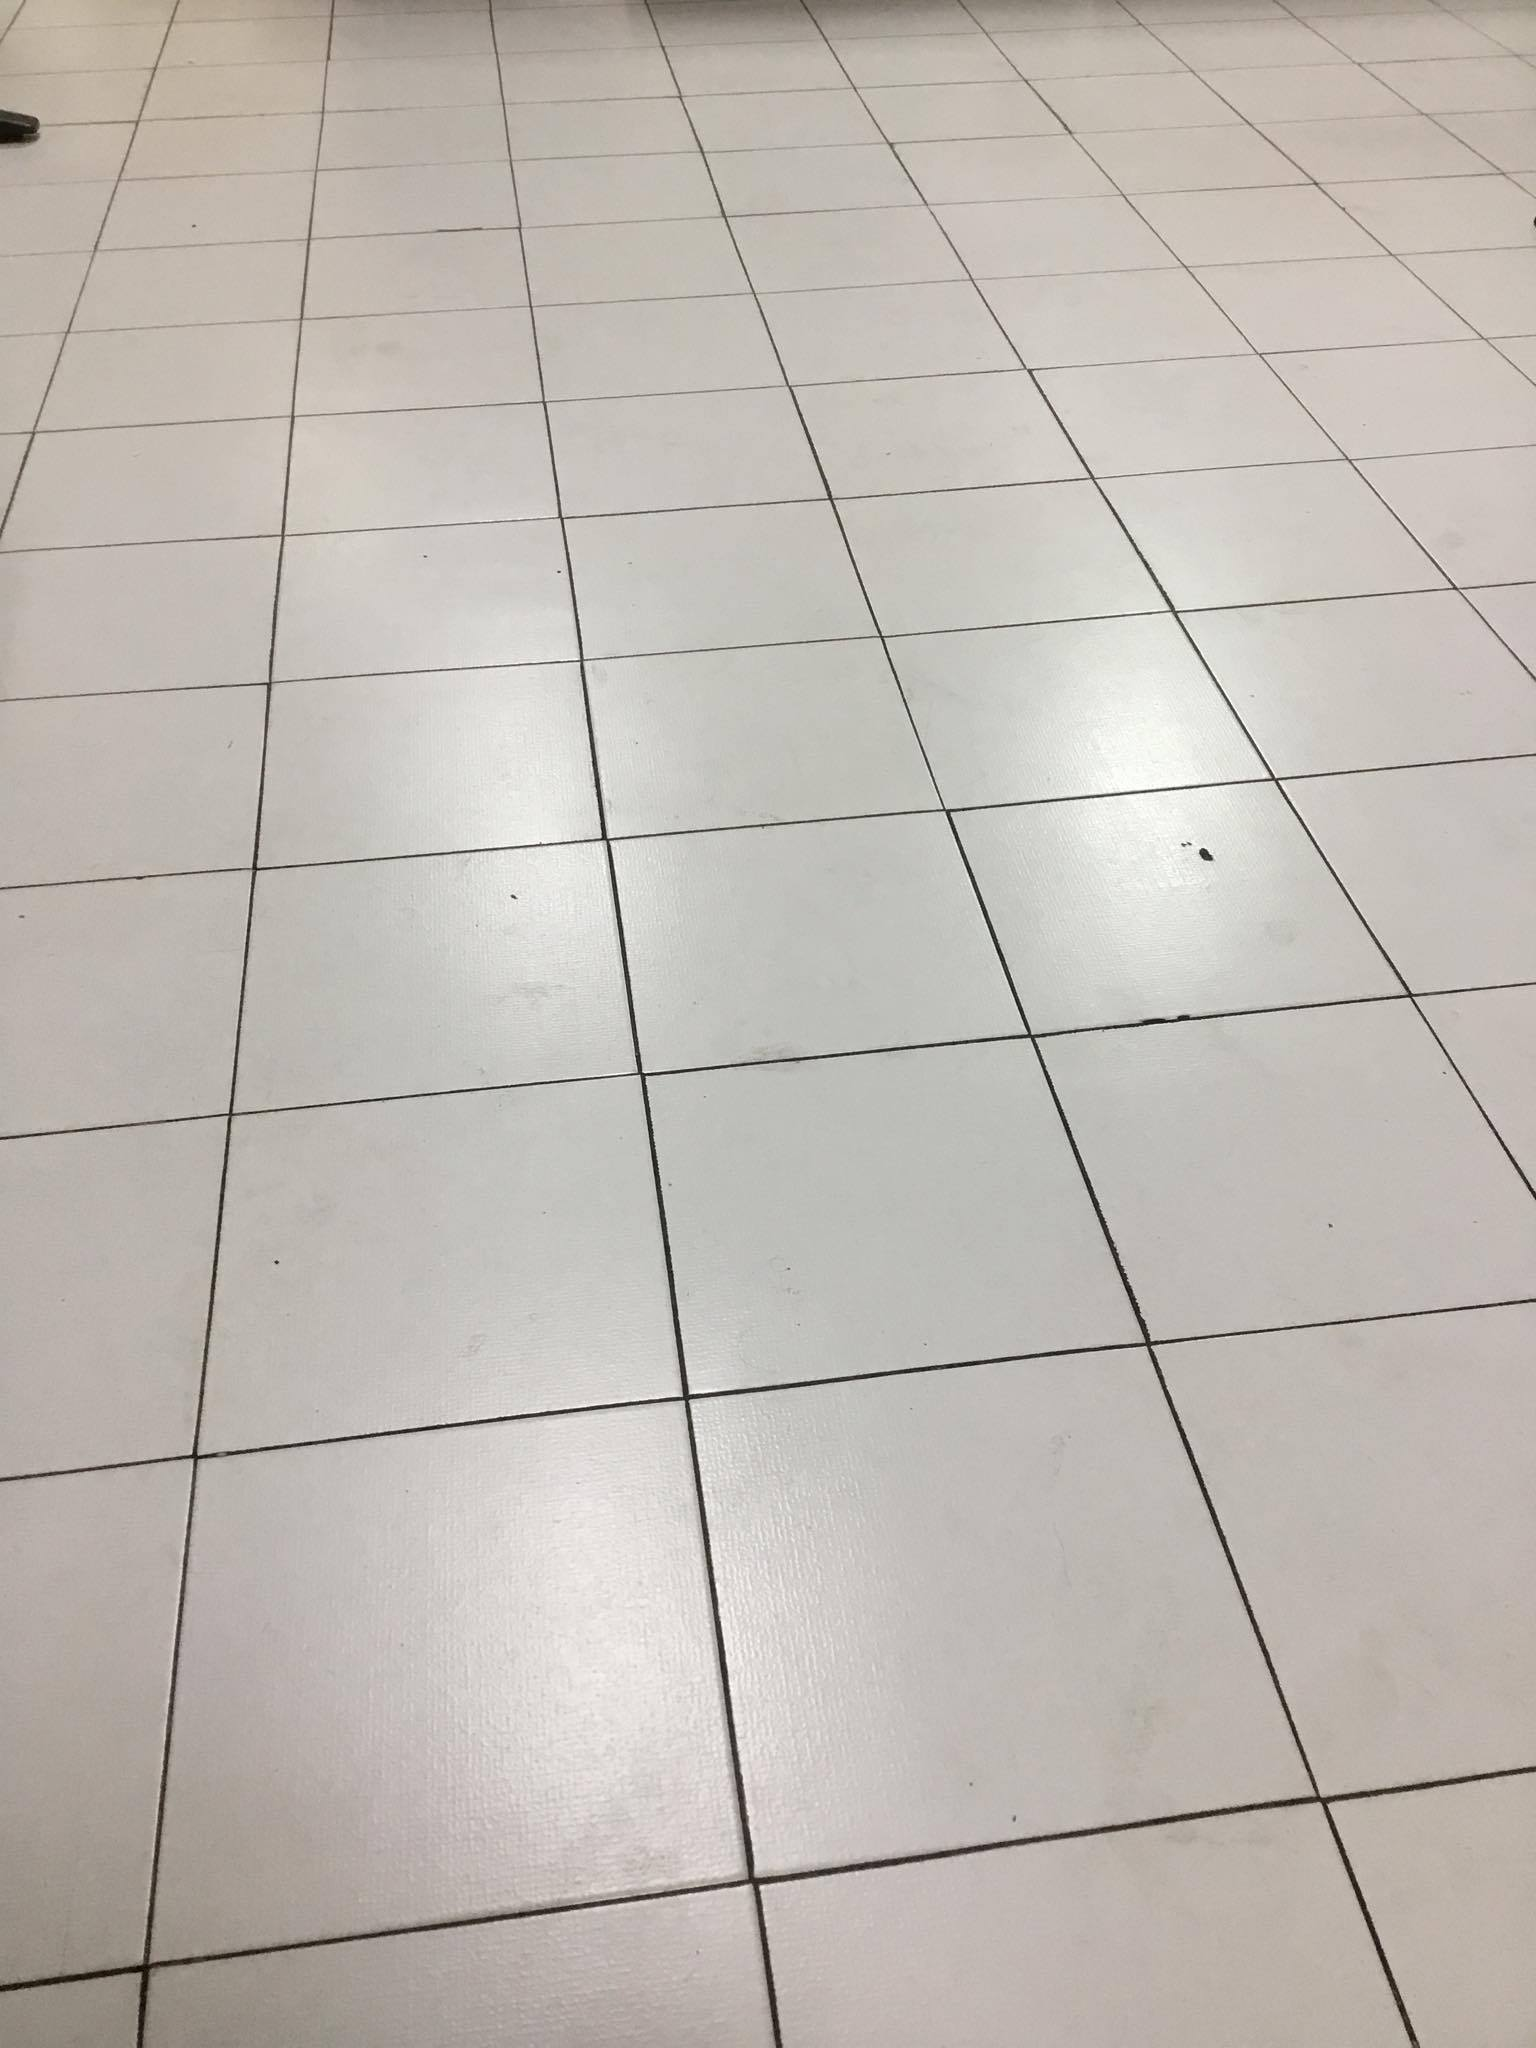
\includegraphics[width=\textwidth]{figures/persp_tile.jpg}
        \caption{Original\label{fig:persp_tile}}    
    \end{subfigure}
    \hfill
    \begin{subfigure}[ht]{0.3\textwidth}  
        \centering 
        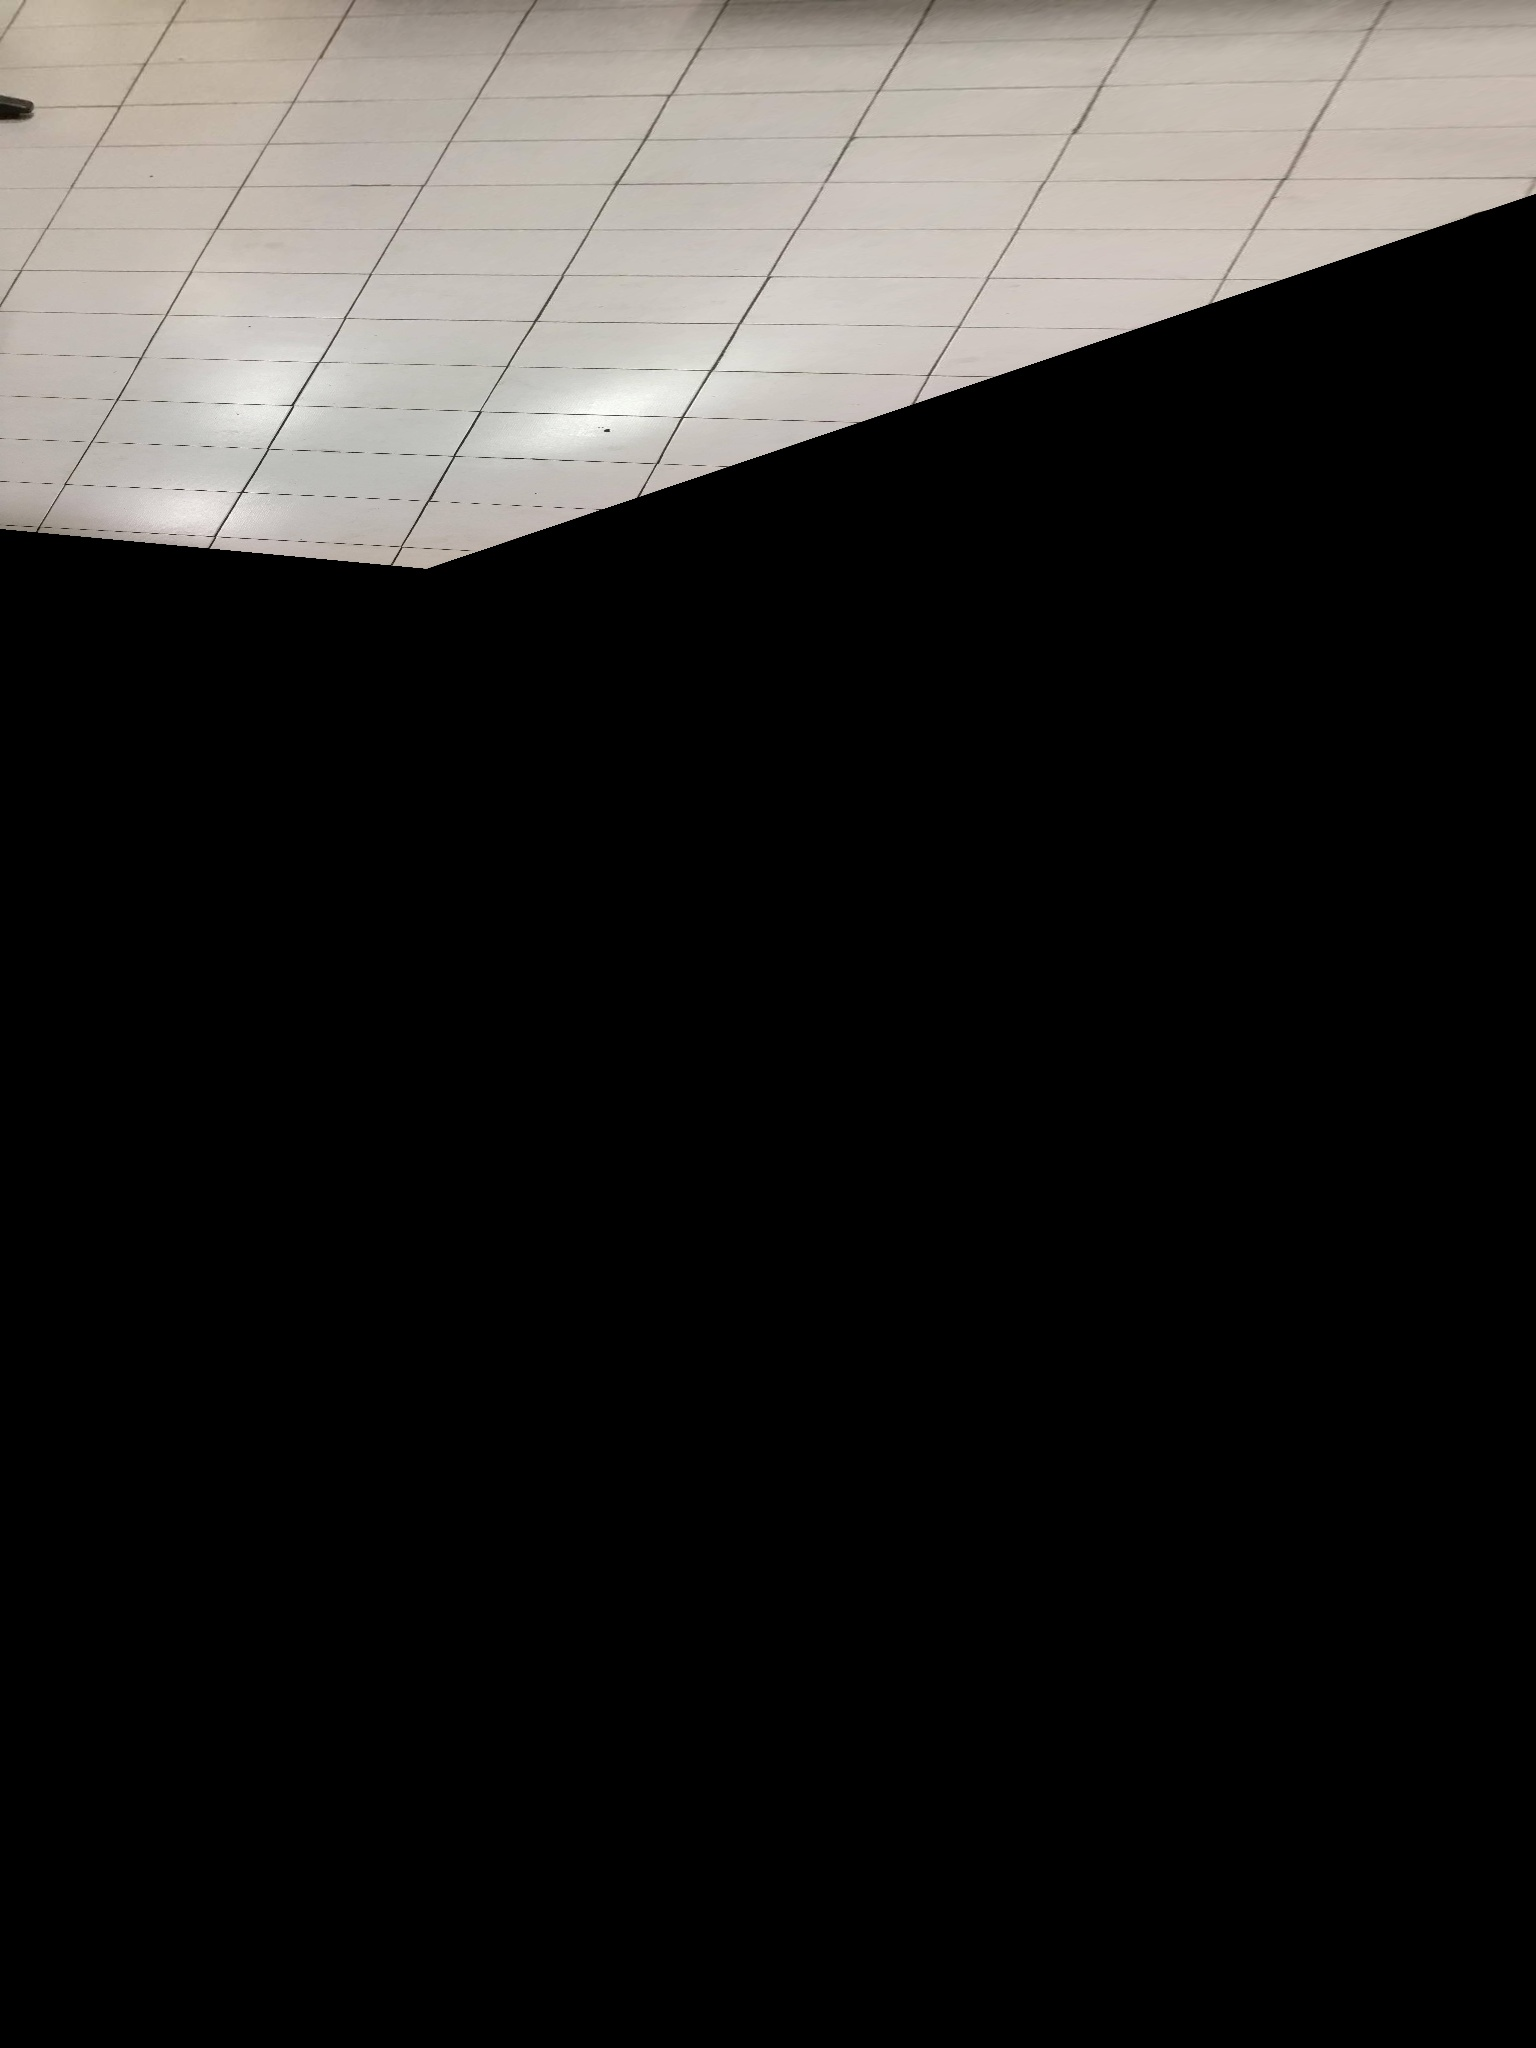
\includegraphics[width=\textwidth]{figures/persp_tile_aff.jpg}
        \caption{Affine\label{fig:persp_tile_aff}}    
    \end{subfigure}
    \hfill
    \begin{subfigure}[ht]{0.3\textwidth}   
        \centering 
        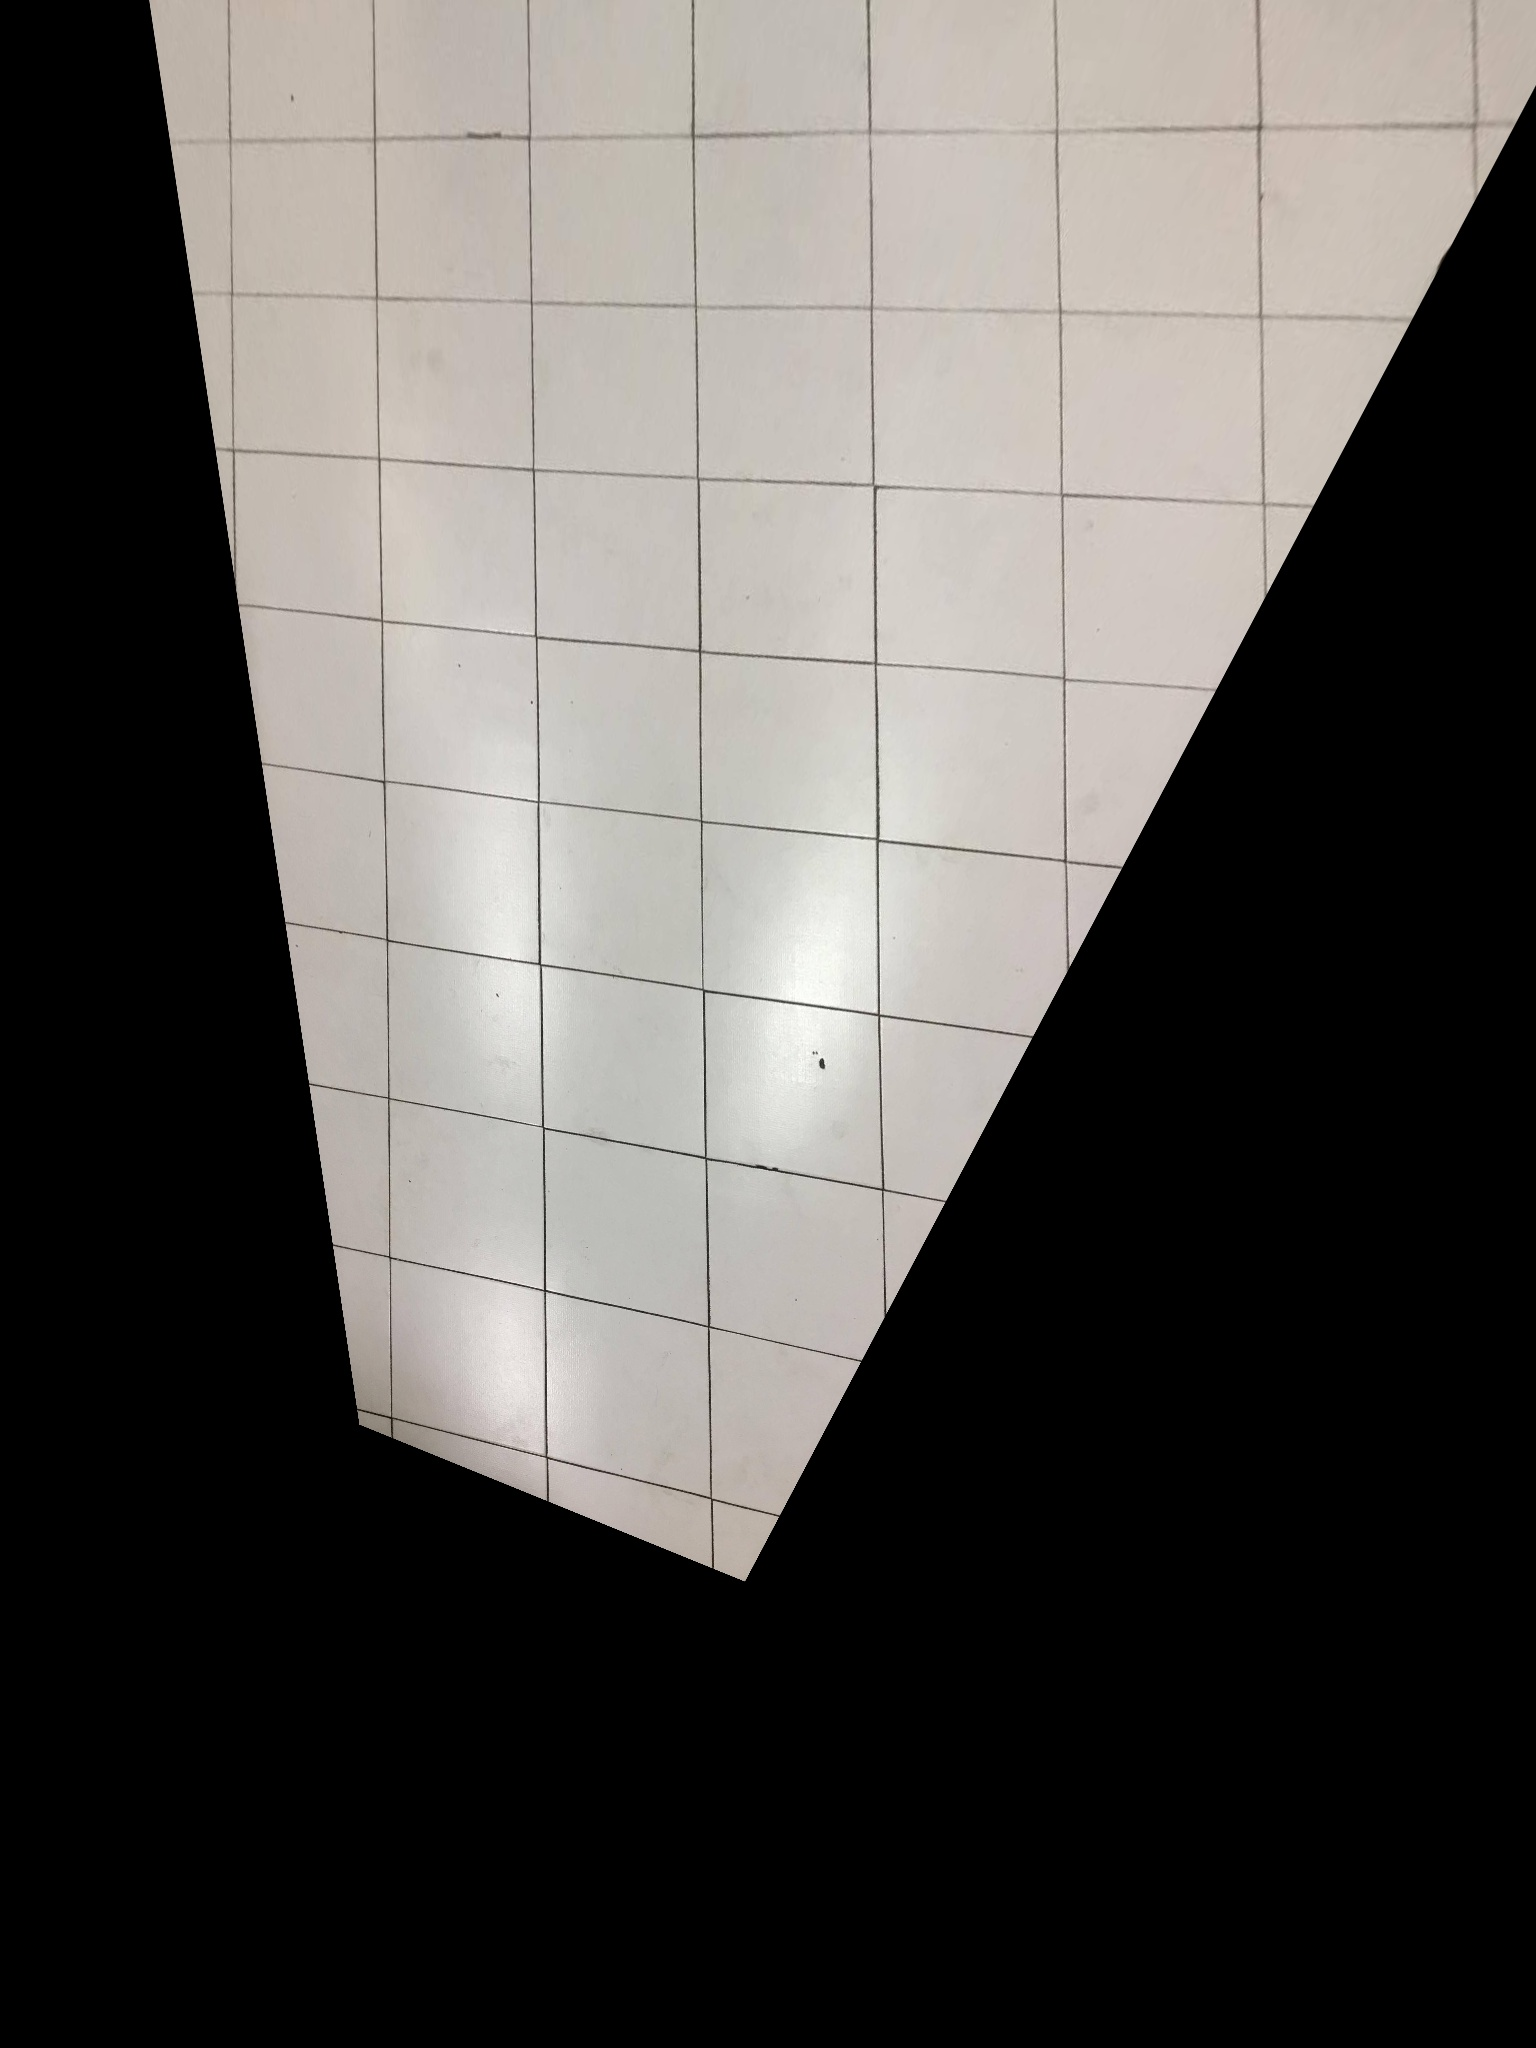
\includegraphics[width=\textwidth]{figures/persp_tile_met.jpg}
        \caption{Metric\label{fig:persp_tile_met}}
    \end{subfigure}

    \vskip \baselineskip

    \centering
    \begin{subfigure}[ht]{0.3\textwidth}
        \centering
        
\includegraphics[width=\textwidth]{figures/img18.jpg}
        \caption{Original\label{fig:img18_tile}}    
    \end{subfigure}
    \hfill
    \begin{subfigure}[ht]{0.3\textwidth}  
        \centering 
        
\includegraphics[width=\textwidth]{figures/img18_aff.jpg}
        \caption{Affine\label{fig:img18_aff}}    
    \end{subfigure}
    \hfill
    \begin{subfigure}[ht]{0.3\textwidth}   
        \centering 
        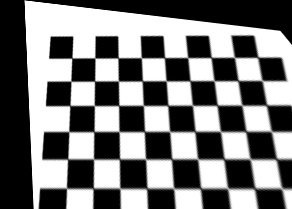
\includegraphics[width=\textwidth]{figures/img18_met.jpg}
        \caption{Metric\label{fig:img18_met}}
    \end{subfigure}

    \vskip \baselineskip
    
    \centering
    \begin{subfigure}[ht]{0.3\textwidth}
        \centering
        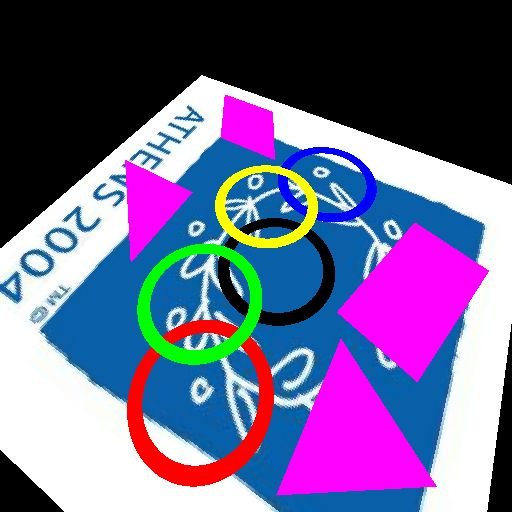
\includegraphics[width=\textwidth]{figures/img11.jpg}
        \caption{Original\label{fig:img11_tile}}    
    \end{subfigure}
    \hfill
    \begin{subfigure}[ht]{0.3\textwidth}  
        \centering 
        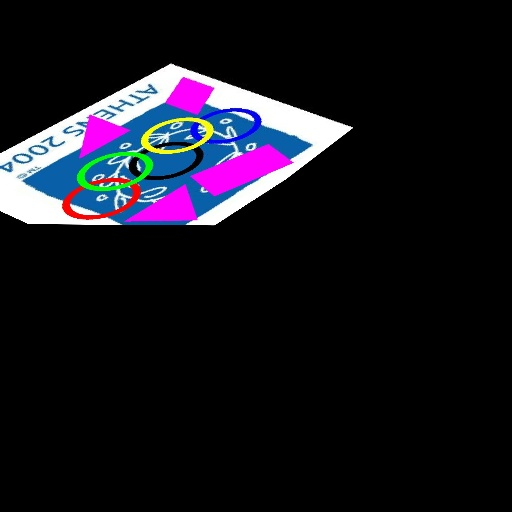
\includegraphics[width=\textwidth]{figures/img11_aff.jpg}
        \caption{Affine\label{fig:img11_aff}}    
    \end{subfigure}
    \hfill
    \begin{subfigure}[ht]{0.3\textwidth}   
        \centering 
        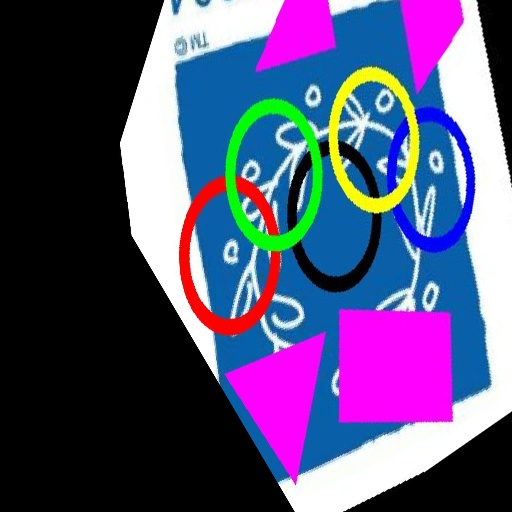
\includegraphics[width=\textwidth]{figures/img11_met.jpg}
        \caption{Metric\label{fig:img11_met}}
    \end{subfigure}
    \caption{Some Sample Results\label{fig:res1}}
\end{figure*}

\begin{figure*}
    \centering
    \begin{subfigure}[ht]{0.3\textwidth}
        \centering
        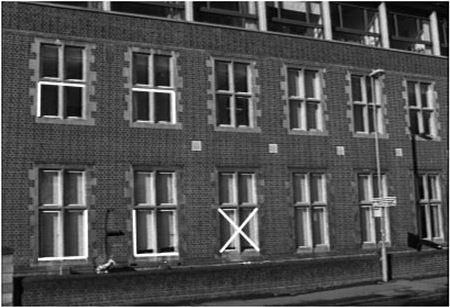
\includegraphics[width=\textwidth]{figures/img16.jpg}
        \caption{Original\label{fig:img16_tile}}    
    \end{subfigure}
    \hfill
    \begin{subfigure}[ht]{0.3\textwidth}  
        \centering 
        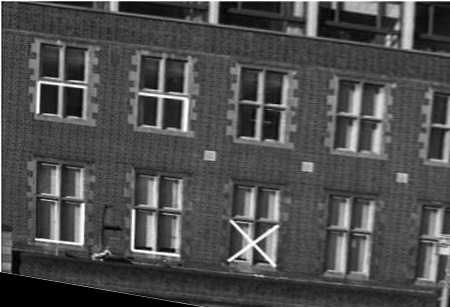
\includegraphics[width=\textwidth]{figures/img16_aff.jpg}
        \caption{Affine\label{fig:img16_aff}}    
    \end{subfigure}
    \hfill
    \begin{subfigure}[ht]{0.3\textwidth}   
        \centering 
        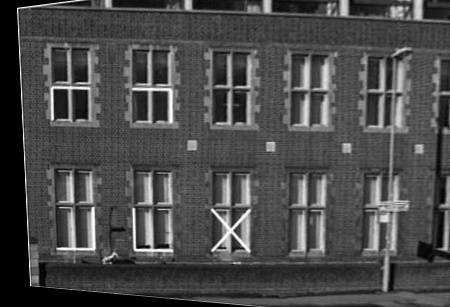
\includegraphics[width=\textwidth]{figures/img16_met.jpg}
        \caption{Metric\label{fig:img16_met}}
    \end{subfigure}

    \vskip \baselineskip

    \centering
    \begin{subfigure}[ht]{0.3\textwidth}
        \centering
        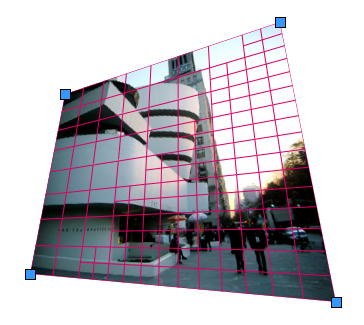
\includegraphics[width=\textwidth]{figures/img14.jpg}
        \caption{Original\label{fig:img14_tile}}    
    \end{subfigure}
    \hfill
    \begin{subfigure}[ht]{0.3\textwidth}  
        \centering
        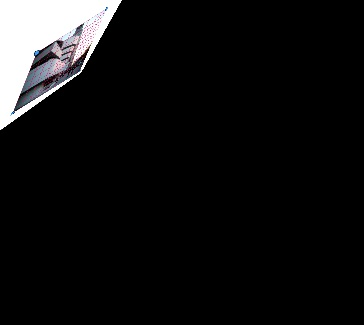
\includegraphics[width=\textwidth]{figures/img14_aff.jpg}
        \caption{Affine\label{fig:img14_aff}}    
    \end{subfigure}
    \hfill
    \begin{subfigure}[ht]{0.3\textwidth}   
        \centering 
        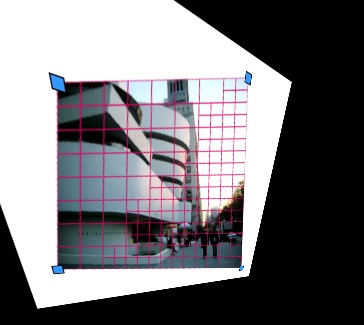
\includegraphics[width=\textwidth]{figures/img14_met.jpg}
        \caption{Metric\label{fig:img14_met}}
    \end{subfigure}
    \caption{Some Sample Results\label{fig:res2}}

    \vskip \baselineskip
    
    \centering
    \begin{subfigure}[ht]{0.3\textwidth}
        \centering
        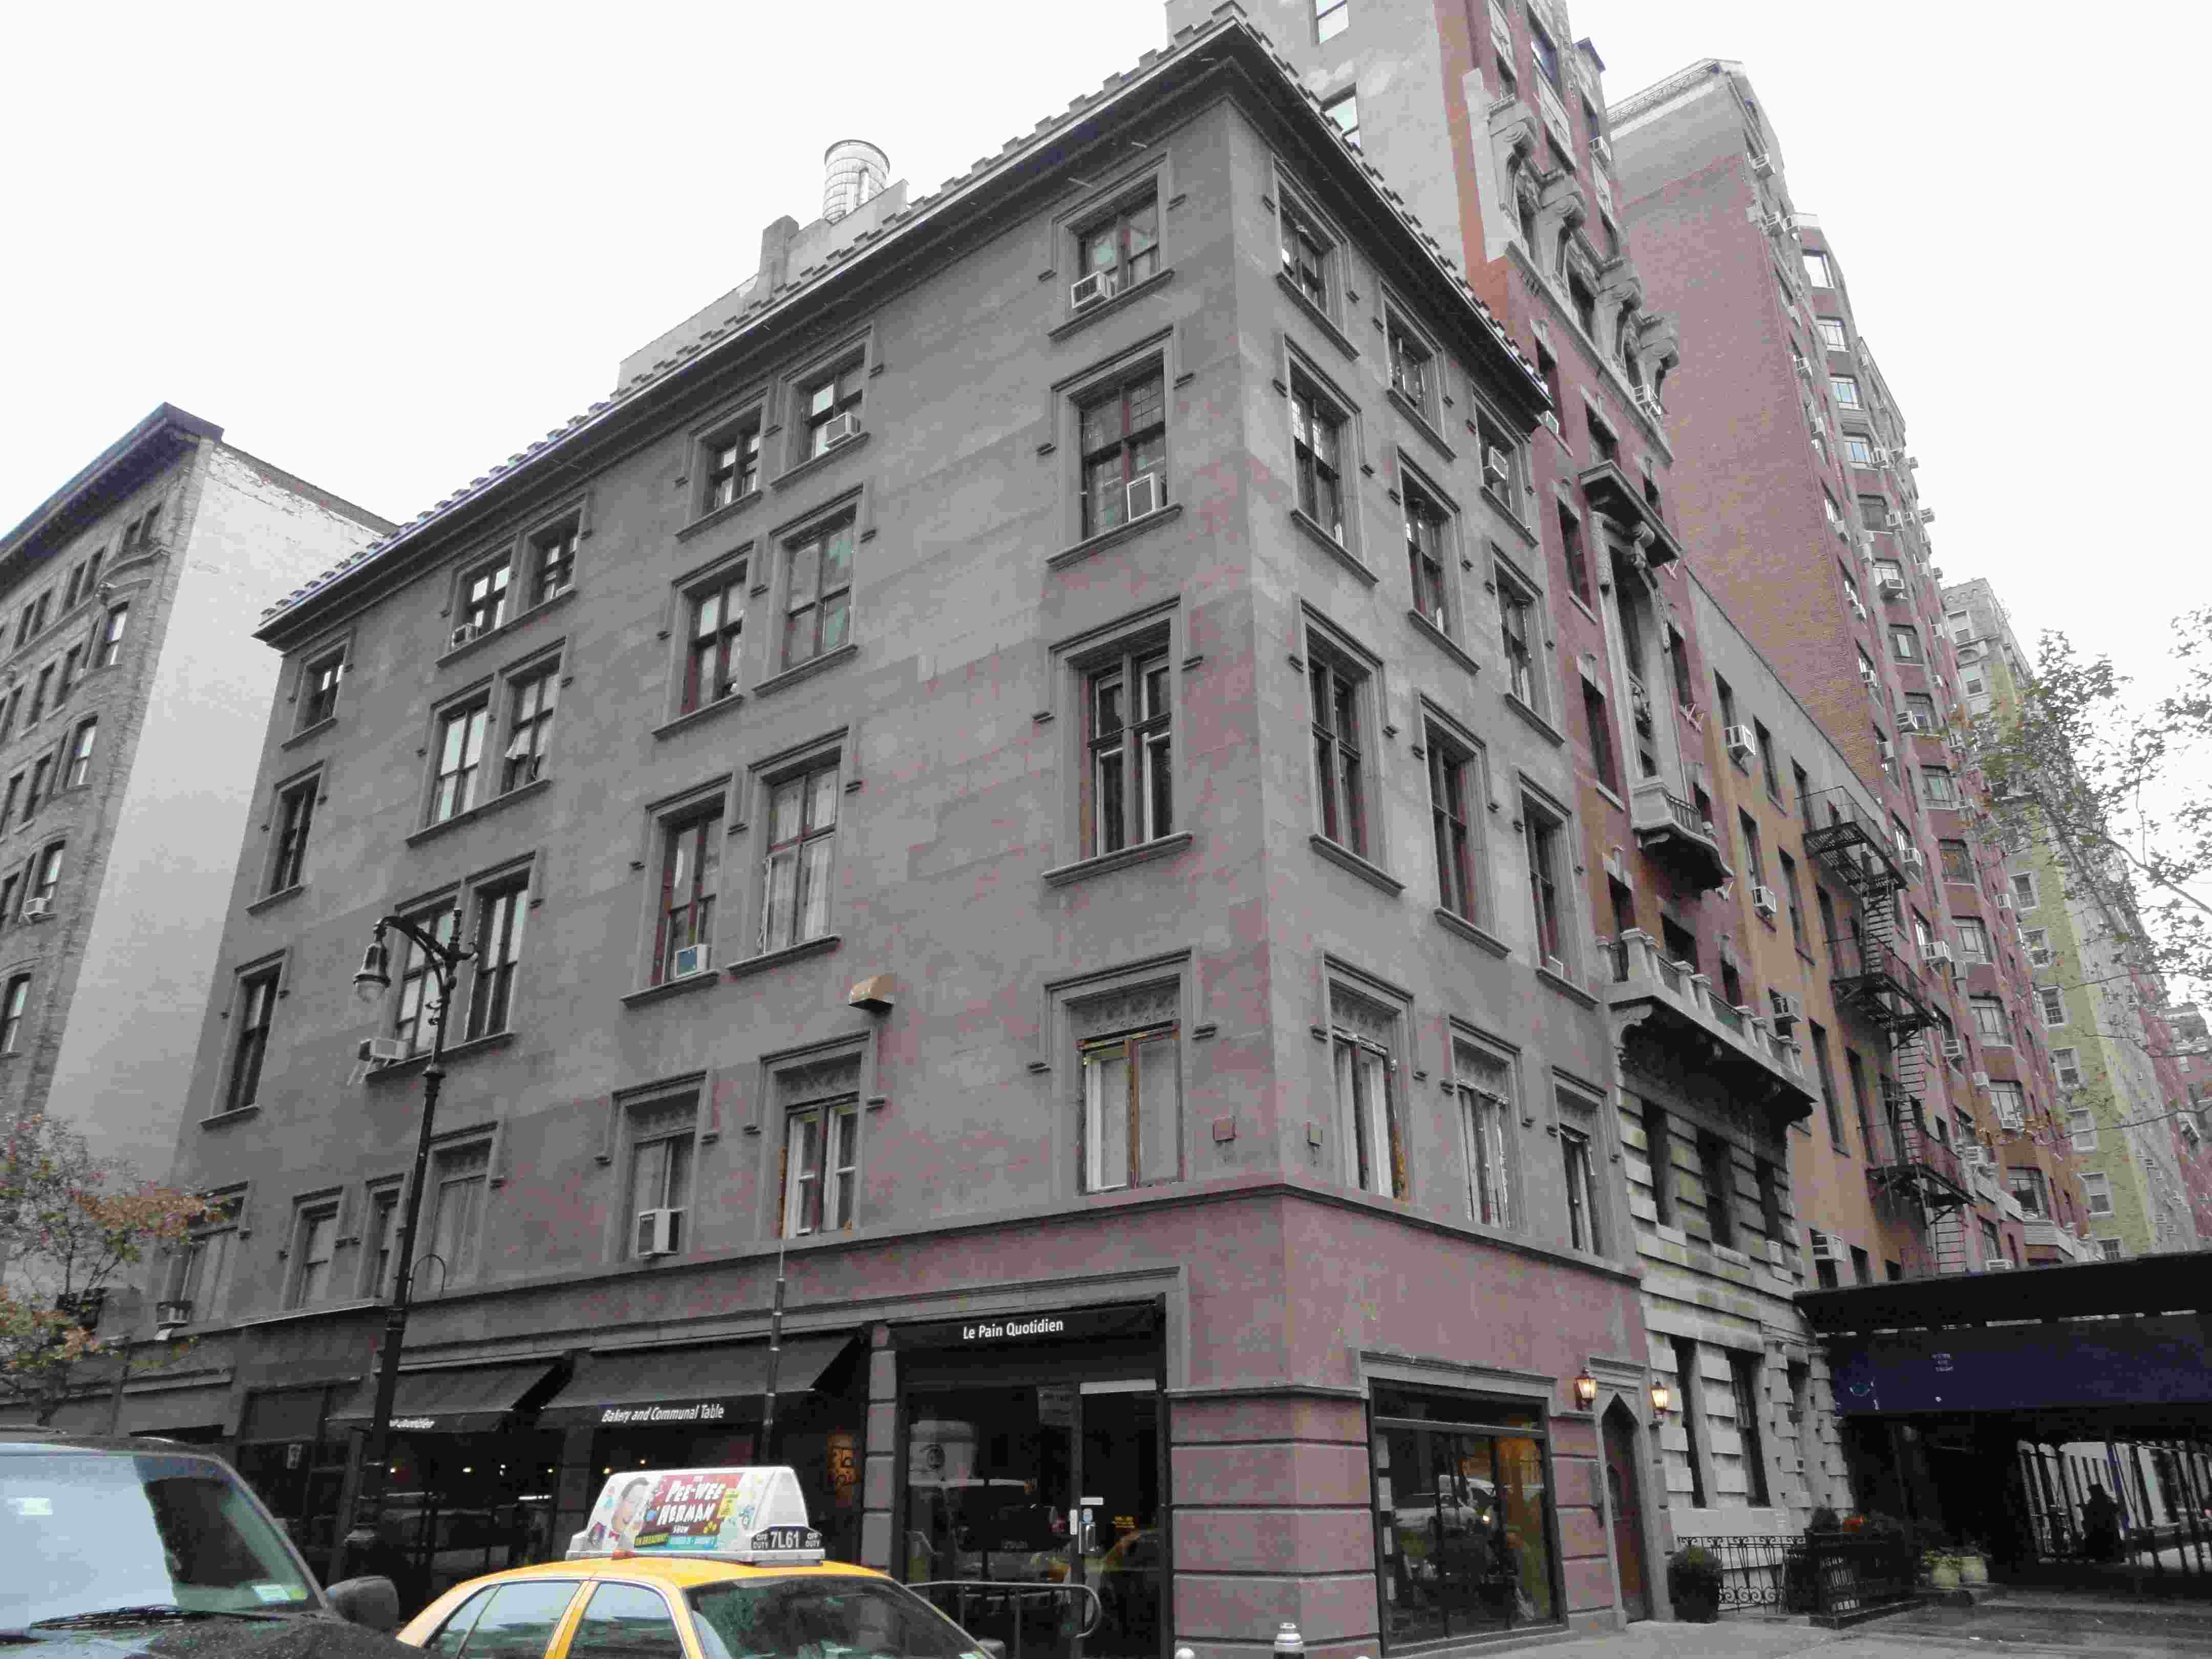
\includegraphics[width=\textwidth]{figures/img3.jpg}
        \caption{Original\label{fig:img3_tile}}    
    \end{subfigure}
    \hfill
    \begin{subfigure}[ht]{0.3\textwidth}  
        \centering
        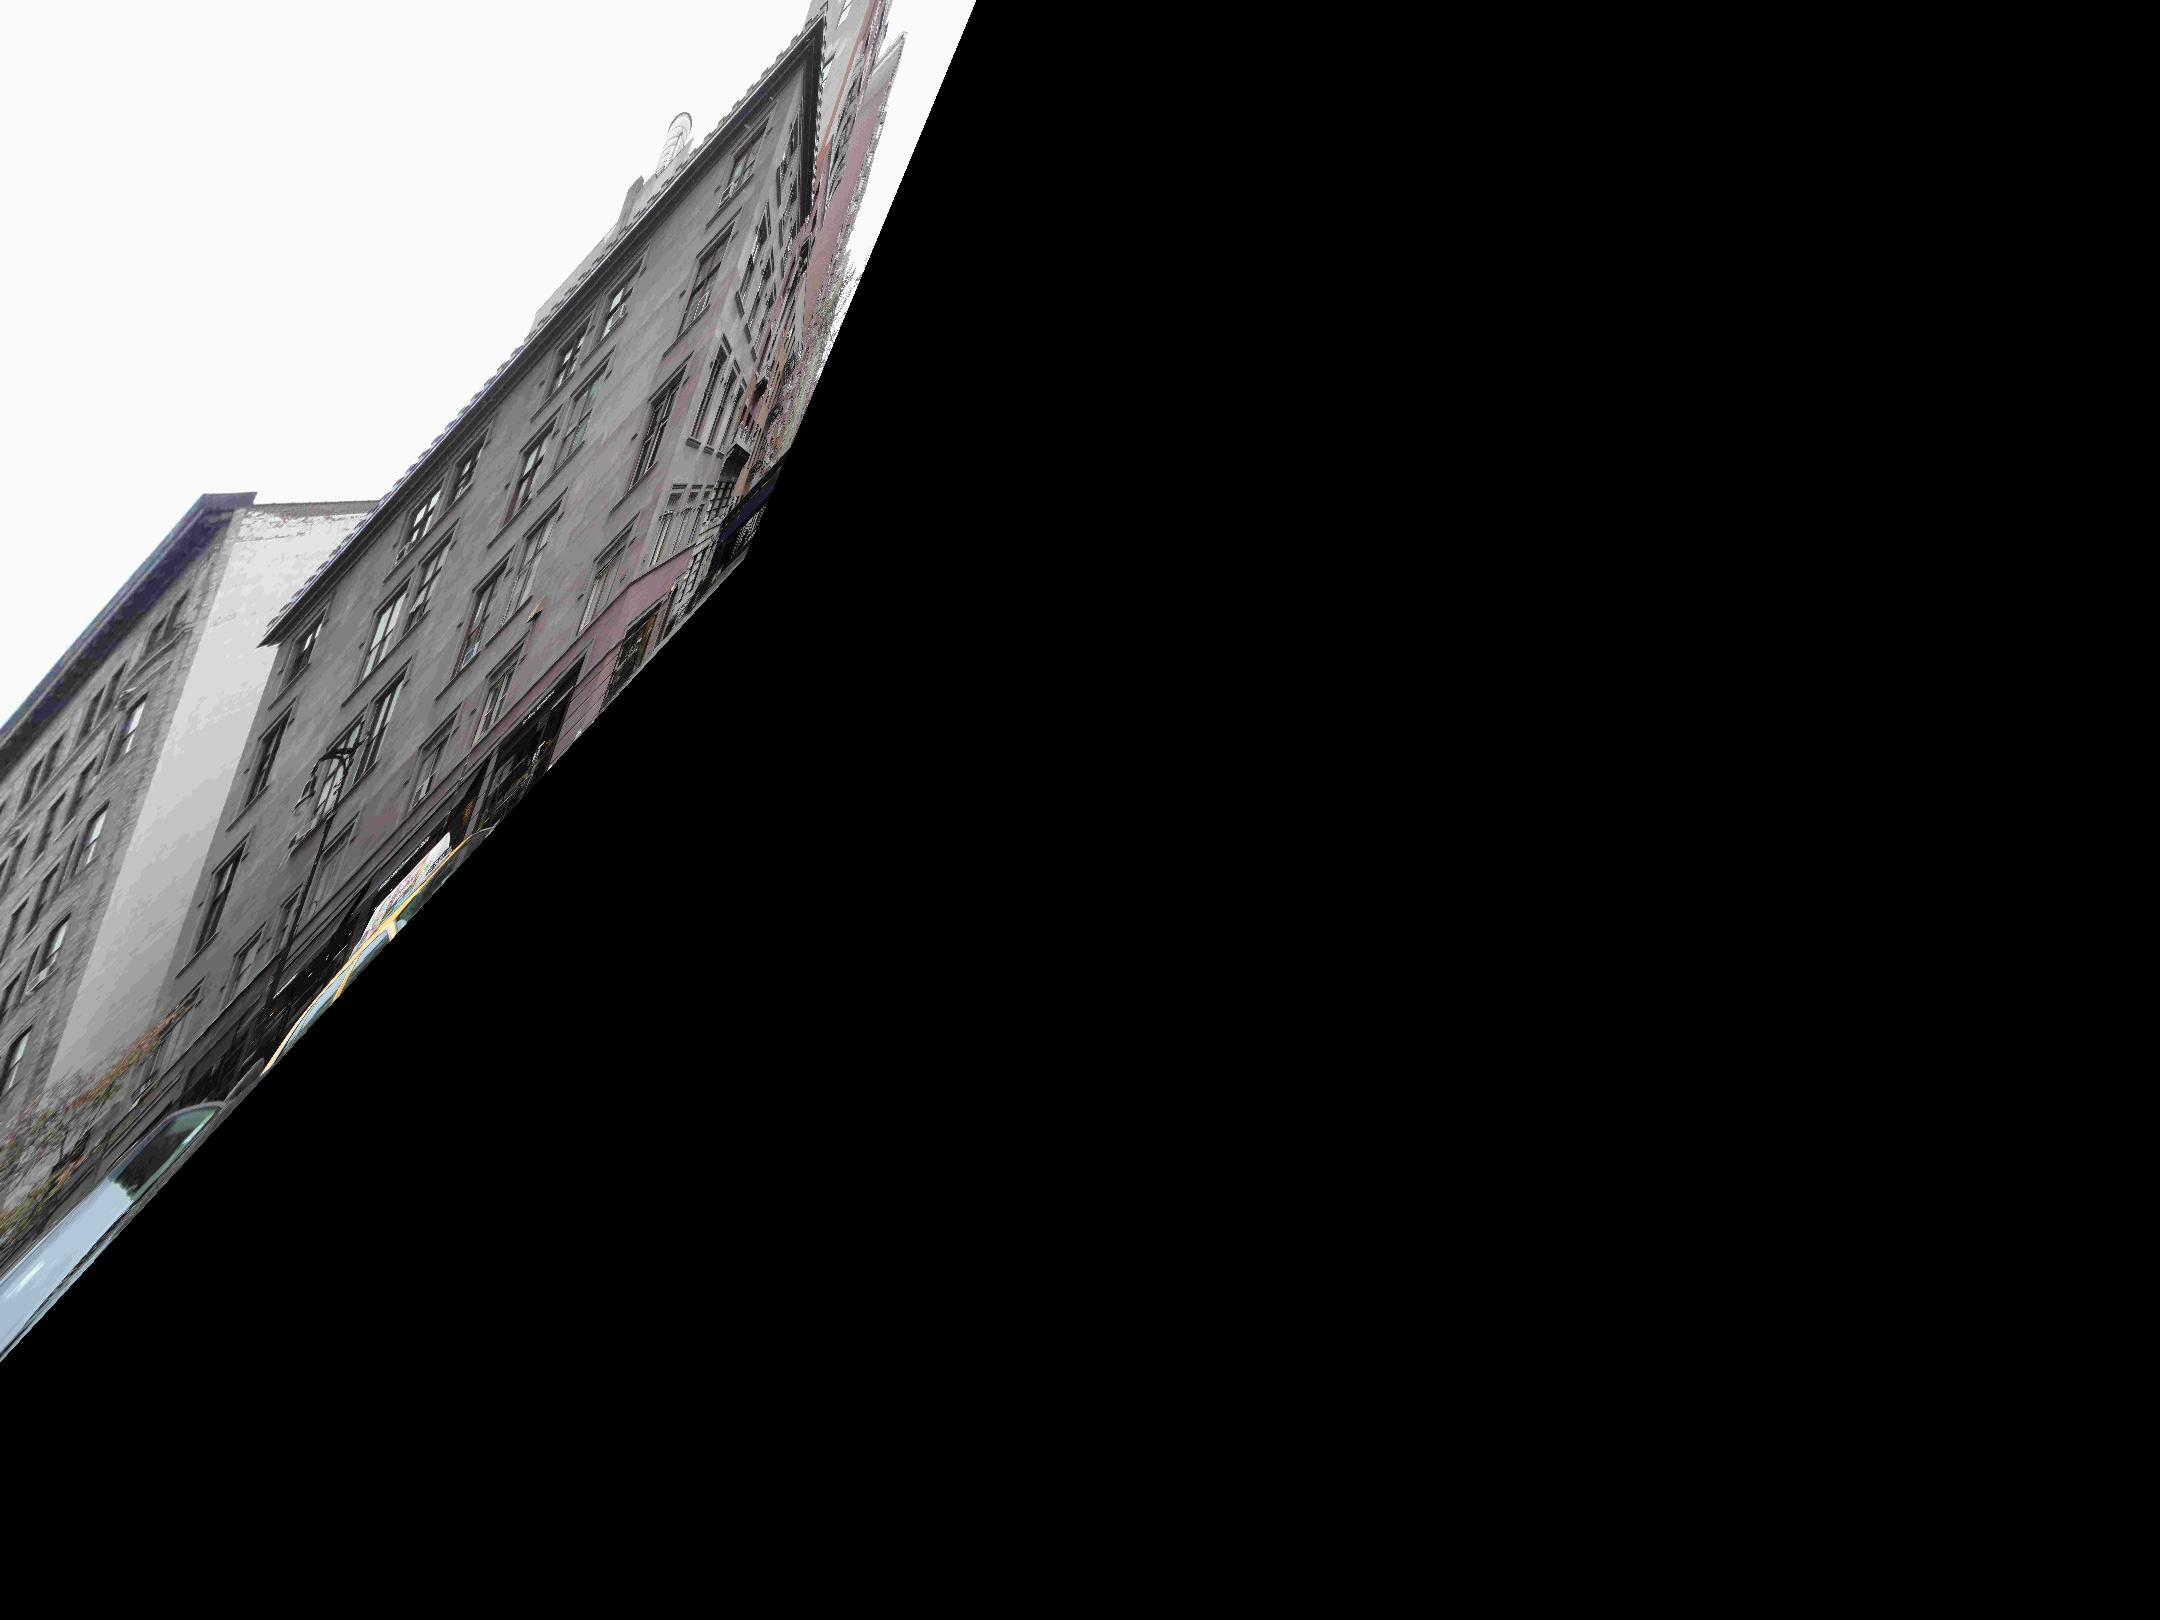
\includegraphics[width=\textwidth]{figures/img3_aff.jpg}
        \caption{Affine\label{fig:img3_aff}}    
    \end{subfigure}
    \hfill
    \begin{subfigure}[ht]{0.3\textwidth}   
        \centering 
        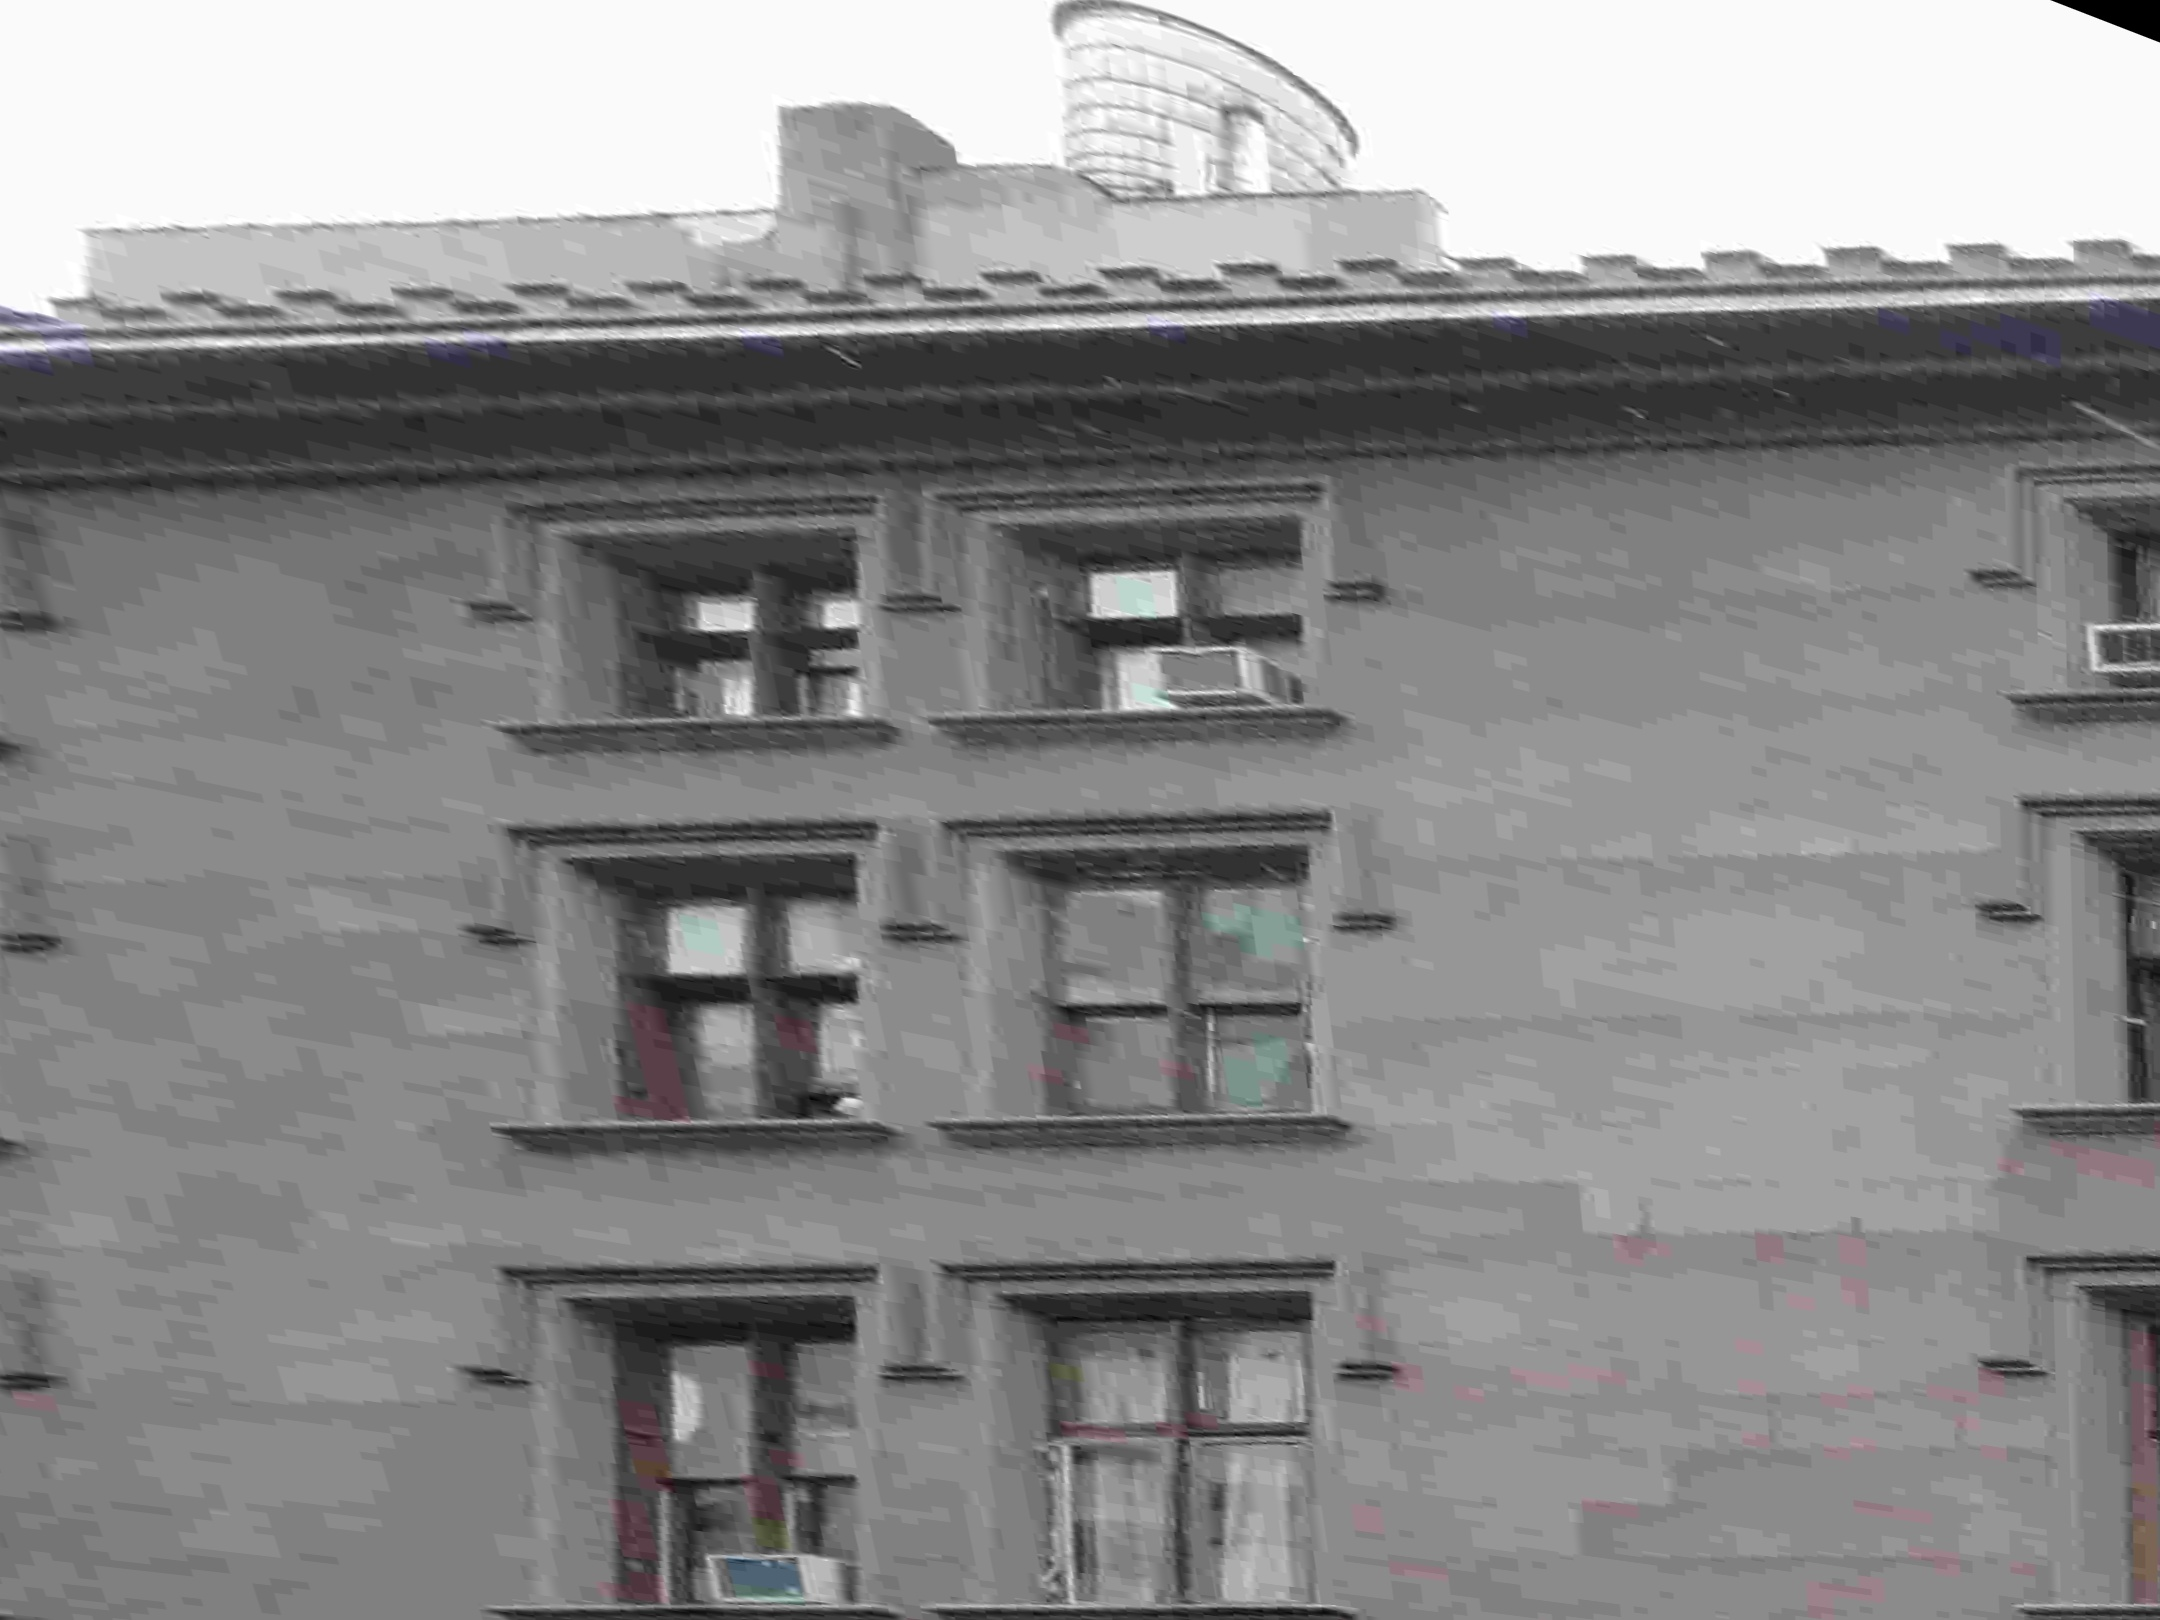
\includegraphics[width=\textwidth]{figures/img3_met.jpg}
        \caption{Metric\label{fig:img3_met}}
    \end{subfigure}
    \caption{Some Sample Results\label{fig:res2}}
\end{figure*}

\end{document}